% Hier folgt der Inhalt des Abschnitts "Ergebnisse und Bewertung".


\subsection{Beispiele Plots und Diagramme}

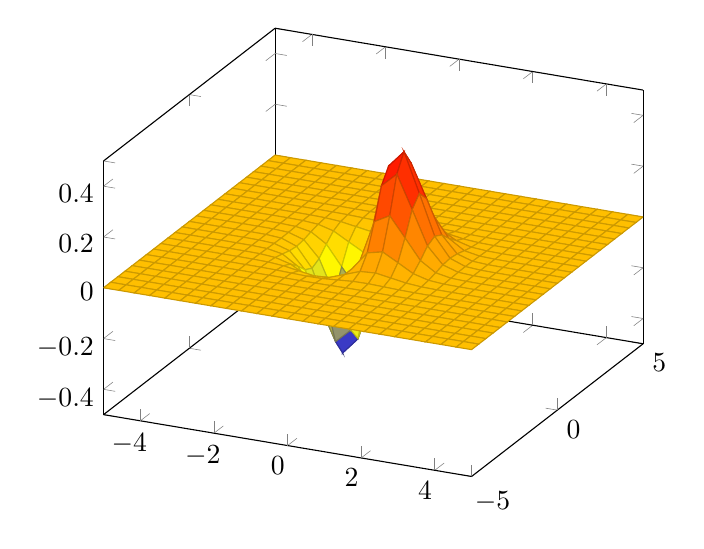
\begin{tikzpicture}
	\begin{axis}
	\addplot3[
			surf,
	]
	{exp(-x^2-y^2)*x};
	\end{axis}
	\end{tikzpicture}

	Plotting from data:

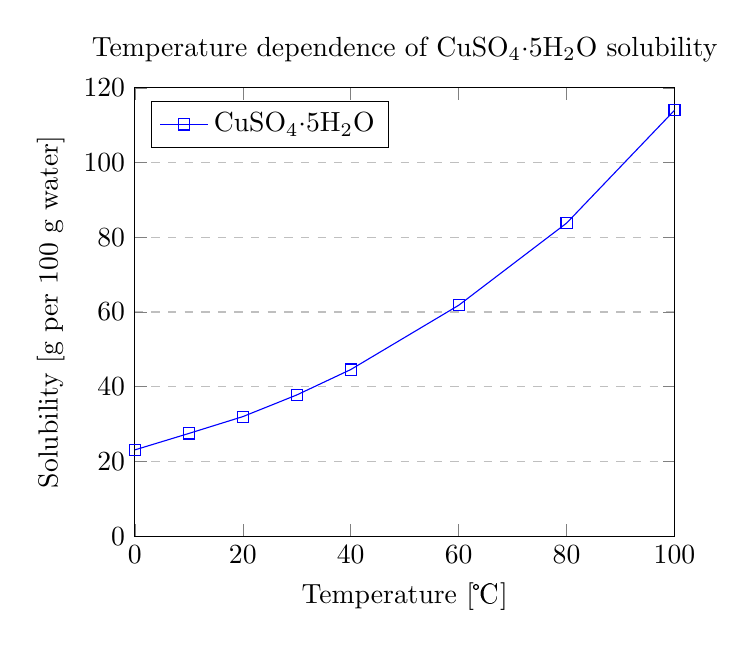
\begin{tikzpicture}
\begin{axis}[
    title={Temperature dependence of CuSO\(_4\cdot\)5H\(_2\)O solubility},
    xlabel={Temperature [\textcelsius]},
    ylabel={Solubility [g per 100 g water]},
    xmin=0, xmax=100,
    ymin=0, ymax=120,
    xtick={0,20,40,60,80,100},
    ytick={0,20,40,60,80,100,120},
    legend pos=north west,
    ymajorgrids=true,
    grid style=dashed,
]

\addplot[
    color=blue,
    mark=square,
    ]
    coordinates {
    (0,23.1)(10,27.5)(20,32)(30,37.8)(40,44.6)(60,61.8)(80,83.8)(100,114)
    };
    \legend{CuSO\(_4\cdot\)5H\(_2\)O}
    
\end{axis}
\end{tikzpicture}

\paragraph*{Info}
Find more examples here: \url{https://www.overleaf.com/learn/latex/Pgfplots_package}
Or here: \url{https://pgfplots.net/}


\section*{Testergebnisse}

\subsection*{Wichtige Metriken}
\begin{itemize}
    \item \textbf{Gesamtanfragen:} 37.900
    \item \textbf{Fehlerrate:} 45,11\% (17.097 Anfragen fehlgeschlagen)
    \item \textbf{Durchschnittliche Antwortzeit:} 66,26 ms
    \item \textbf{Erfolgsquote Registrierung:} 9\% (927 von 9.475 Iterationen erfolgreich)
    \item \textbf{Erfolgsquote Rezeptverwaltung:} 9\% (926 von 9.475 Iterationen erfolgreich)
\end{itemize}

\subsection*{Antwortzeiten}
\begin{figure}
    \centering
    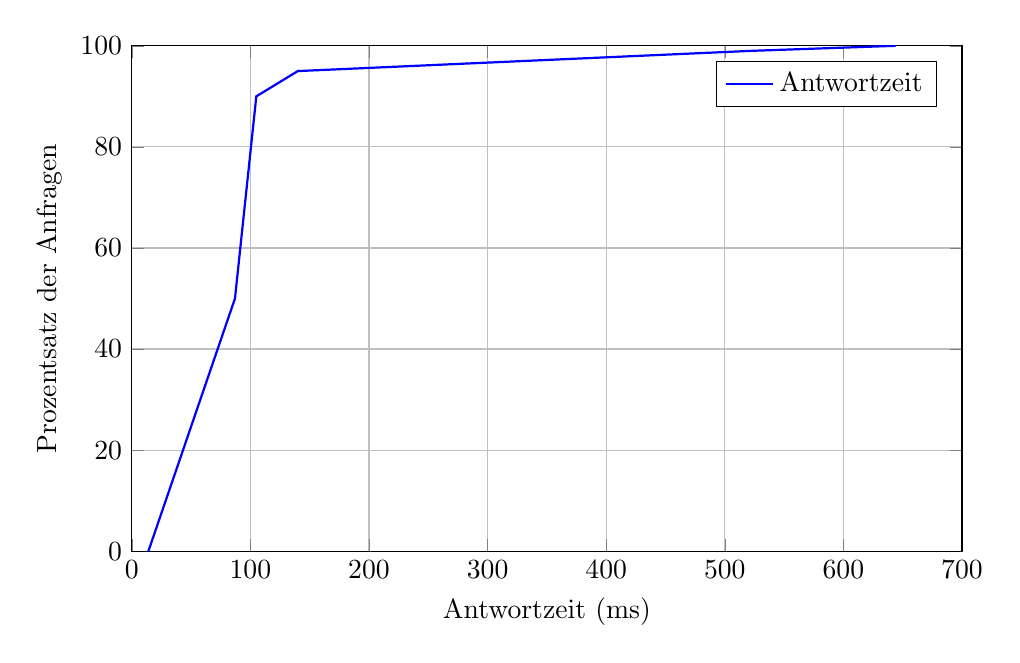
\begin{tikzpicture}
        \begin{axis}[
            width=\textwidth,
            height=8cm,
            xlabel={Antwortzeit (ms)},
            ylabel={Prozentsatz der Anfragen},
            ymin=0, ymax=100,
            xmin=0, xmax=700,
            xtick={0,100,200,300,400,500,600,700},
            ytick={0,20,40,60,80,100},
            legend pos=north east,
            grid=both,
            ]
            \addplot[blue, thick] coordinates {
                (14, 0) (87, 50) (105, 90) (140, 95) (522, 99) (644, 100)
            };
            \addlegendentry{Antwortzeit}
        \end{axis}
    \end{tikzpicture}
    \caption{Antwortzeiten der API (90. Perzentil: 105 ms, 95. Perzentil: 140 ms)}
    \label{fig:response_time}
\end{figure}

\subsection*{Erfolgsquoten der Checks}
\begin{figure}
    \centering
    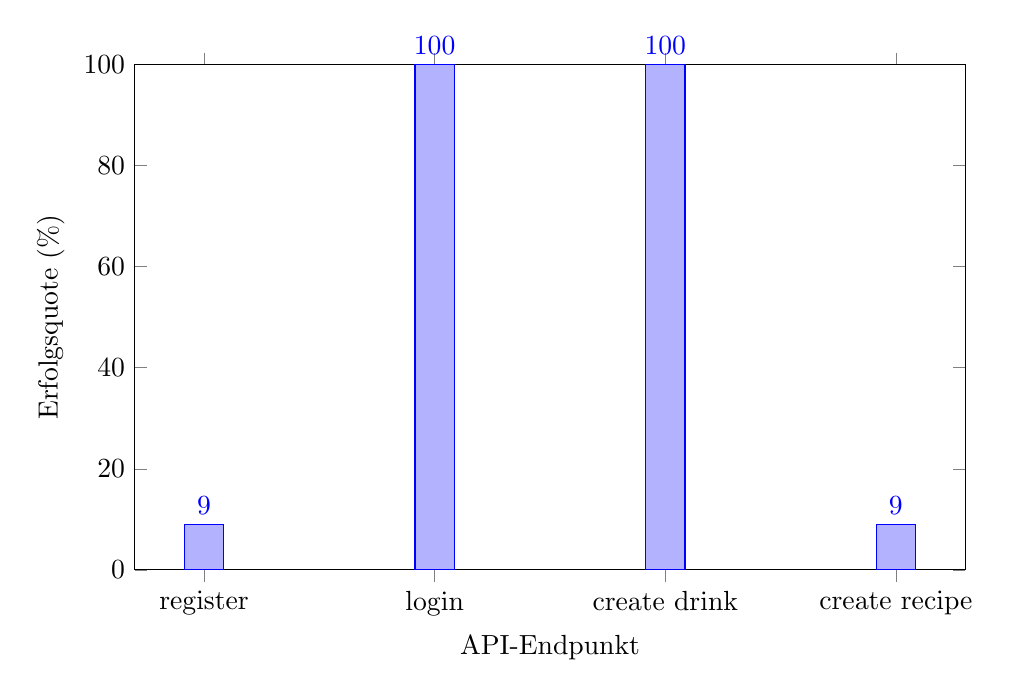
\begin{tikzpicture}
        \begin{axis}[
            ybar,
            width=\textwidth,
            height=8cm,
            xlabel={API-Endpunkt},
            ylabel={Erfolgsquote (\%)},
            ymin=0, ymax=100,
            symbolic x coords={register, login, create drink, create recipe},
            xtick=data,
            bar width=0.5cm,
            nodes near coords,
            nodes near coords align={vertical},
            ]
            \addplot coordinates {(register, 9) (login, 100) (create drink, 100) (create recipe, 9)};
        \end{axis}
    \end{tikzpicture}
    \caption{Erfolgsquoten der Haupt-API-Endpunkte}
    \label{fig:success_rates}
\end{figure}

\subsection*{Fehlerrate über die Zeit}
\begin{figure}
    \centering
    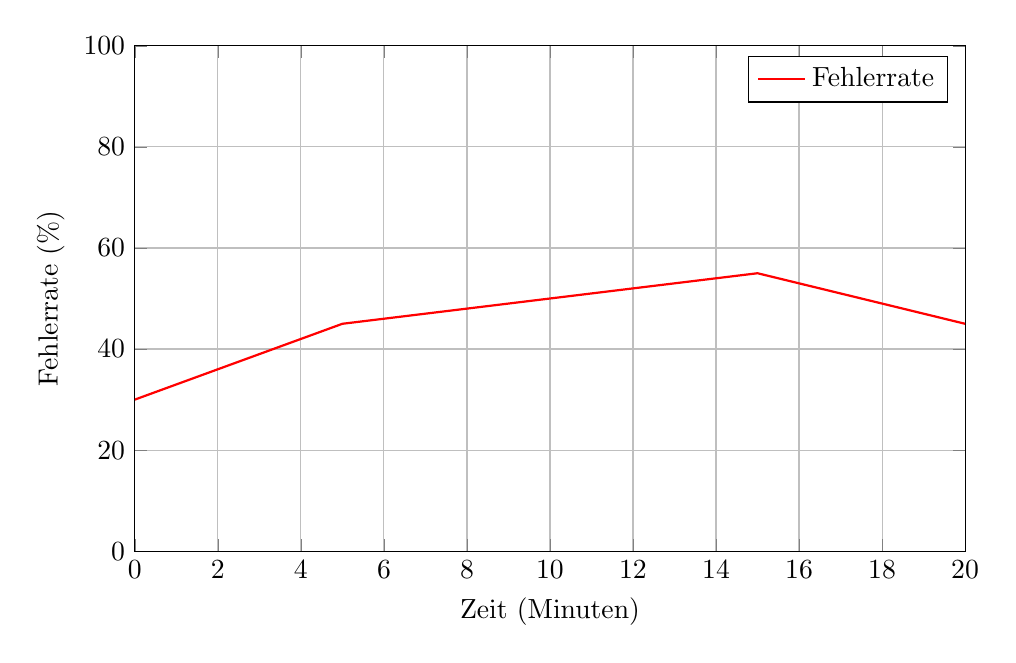
\begin{tikzpicture}
        \begin{axis}[
            width=\textwidth,
            height=8cm,
            xlabel={Zeit (Minuten)},
            ylabel={Fehlerrate (\%)},
            xmin=0, xmax=20,
            ymin=0, ymax=100,
            grid=both,
            ]
            \addplot[red, thick] coordinates {
                (0, 30) (5, 45) (10, 50) (15, 55) (20, 45)
            };
            \addlegendentry{Fehlerrate}
        \end{axis}
    \end{tikzpicture}
    \caption{Fehlerrate im Verlauf des Tests}
    \label{fig:error_rate}
\end{figure}

\section*{Schlussfolgerungen}
Die Ergebnisse zeigen, dass:
\begin{itemize}
    \item Die Benutzerregistrierung und Rezeptverwaltung besonders fehleranfällig sind (nur 9\% Erfolgsquote).
    \item Die API insgesamt eine hohe Fehlerrate von 45,11\% aufweist, was auf Skalierungs- oder Ressourcenprobleme hindeuten könnte.
    \item Die durchschnittliche Antwortzeit (66,26 ms) akzeptabel ist, aber in Spitzenzeiten (max. 644 ms) stark ansteigt.
\end{itemize}

\section*{Empfehlungen}
\begin{itemize}
    \item Optimieren Sie die Ressourcen- und Skalierungseinstellungen von Google Cloud Run.
    \item Reduzieren Sie die Last in der Benutzerregistrierung durch bessere Datenbankabfragen oder asynchrone Prozesse.
    \item Testen Sie kleinere Benutzergruppen, um die Schwellenwerte für Stabilitätsprobleme zu identifizieren.
\end{itemize}